\subsection{Memento}

\subsubsection{Objetivo}

Sem violar o encapsulamento, capturar e externalizar o estado interno de um objeto de modo a que o mesmo possa ser reposto posteriormente.

\subsubsection{Motivação}

Considere-se por exemplo um editor gráfico que permite definir linhas entre rectângulos e que quando se desloca um dos rectângulos a linha altera-se apropriadamente:

\centerline{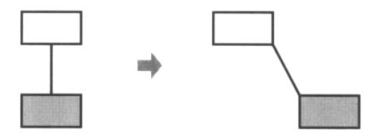
\includegraphics[scale=.7]{img/memento/motivation.png}}

Uma forma recorrente de realizar este tipo de operação é através de um sistema especializado, cuja funcionalidade é encapsulada num objeto (ConstraintSolver).

Por forma a suportar a operação undo, é necessário guardar registos dos vários estados do objeto ContraintSolver. Isto pode ser feito à custa de um memento (SolverState), um objeto que armazena um snapshot do estado interno de outro objeto (originador).

\subsubsection{Aplicação}

Usar quando:
\begin{itemize}
\item é necessário manter registos do estado de um objeto por forma a ser possível repô-lo mais tarde;
\item não é possível expor esse estado através de getters.
\end{itemize}

\subsubsection{Estrutura}

\centerline{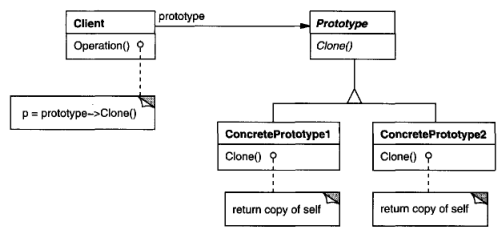
\includegraphics[scale=.7]{img/memento/structure.png}}

\subsubsection{Participantes}
\begin{itemize}
\item Memento (SolverState), guarda o estado do objeto Originator e não disponibiliza esse estado a outros objetos para além do originador
\item Originator (ConstraintSolver), cria o memento e usa-o para repor o seu estado interno
\item Caretaker, é o responsável pelo mecanismo de undo
\end{itemize}

\subsubsection{Colaborações}

\begin{itemize}
\item O caretaker requisita um memento ao originador, mantém-no durante algum tempo, e devolve-o ao originador:

\centerline{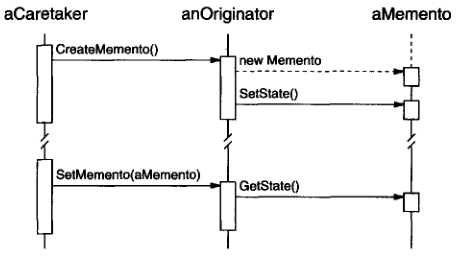
\includegraphics[scale=.7]{img/memento/caretaker.png}}

\item O memento é passivo, apenas o originador que o criou atribui ou recupera o seu estado.
\end{itemize}

\subsubsection{Consequências}
\begin{itemize}
\item Garante a preservação do encapsulamento do Originator.
\item Simplifica a classe Originator, pois esta não necessita de gerir as versões do seu estado interno.
\item Pode implicar um elevado overhead.
\item Aumento do uso de memória para manter os vários mementos.
\end{itemize}

\subsubsection{Implementação}
\begin{itemize}
\item Quando se cria um memento, este não deve guardar todo o estado mas apenas as alterações relativamente ao último snapshot.
\end{itemize}